\chapter{RESEARCH METHODOLOGY}
\label{ch:methodology}

% Describe how the study was conducted, well enough for someone else to
% reproduce it. This chapter is the bulk of the report (~1,500-2,500 words).
% The "Use of AI Tools" subsection at the END is MANDATORY per handbook \S1.1.

\section{System Overview}
\label{sec:method:overview}

% One paragraph describing the modular monolith - data loader, embedding
% pipeline, engines, storage, API+UI. Reference Figure \ref{fig:architecture}.

The system is a modular monolith that performs cross-modal retrieval: given a
short text query such as ``a dog on a beach'', it returns the dataset images
whose content best matches that description. Text and images are never compared
directly. Instead, the same embedding model maps both into a shared vector
space, and retrieval becomes the problem of finding the dataset vectors closest
to the query vector. The defining property of the system is that the component
performing this closest-vector search is interchangeable. A classical engine, a
quantum engine, and a hybrid of the two all expose one common interface, so a
single query can be answered by any of them and the rankings placed side by
side. This makes the system an instrument for comparing search strategies
rather than a single retrieval product.\footnote{The full source code, benchmark
harness, and dataset configuration are publicly available at
\url{https://github.com/Mirza404/quantum-vector-search}.}

This interchangeability is enforced by a single design decision that runs
through the whole codebase: the strategy pattern. Each stage of the pipeline is
defined by an abstract interface, and concrete implementations plug into it.
Data loaders implement \texttt{BaseDataLoader}, embedding models implement
\texttt{EmbeddingGenerator}, and every search engine implements
\texttt{SearchEngineStrategy}, which requires just two operations,
\texttt{build\_index} and \texttt{search}. Because all engines satisfy the same
contract, the surrounding harness that loads data, generates embeddings, runs
queries, and records results is identical for every engine. Any difference we
measure between a classical and a quantum engine therefore reflects the engine
itself, not the code around it. Which engines run, at which vector dimensions,
and with how many measurement shots is selected in a configuration file
(\texttt{benchmarks.yaml}) rather than by editing source, so an experiment is
defined by configuration rather than by code changes.

The pipeline is organised into five phases, shown in
Figure~\ref{fig:architecture}. In the first phase, data loading, a
\texttt{DirectoryDataLoader} reads the image files and the accompanying
ground-truth pairs that define which image each query should retrieve. In the
second phase, the embedding pipeline, a CLIP model converts every image and
every text query into a vector. In the third phase the search engines build
their indexes over these vectors and answer queries, each engine applying its
own strategy, whether classical, quantum, or hybrid. In the fourth phase the
outcome of every run, including its accuracy and resource measurements, is
written to a PostgreSQL database. The fifth phase exposes the system through a
FastAPI backend and a React interface, which lets a user issue a query and
inspect the rankings returned by each engine. The sections that follow describe
each phase in turn: the dataset and ground truth in
Section~\ref{sec:method:dataset}, the embedding pipeline in
Section~\ref{sec:method:embeddings}, and the individual search engines in
Section~\ref{sec:method:engines}.

\begin{figure}[ht]
  \centering
  \begin{tikzpicture}[
      font=\small,
      box/.style={draw, rounded corners, align=center, inner sep=5pt,
        text width=58mm, fill=gray!8},
      eng/.style={draw, rounded corners, align=center, inner sep=4pt,
        text width=30mm, minimum height=12mm, font=\footnotesize},
      classical/.style={eng, fill=blue!10, draw=blue!55},
      quantum/.style={eng, fill=violet!12, draw=violet!55},
      hybrid/.style={eng, fill=green!12, draw=green!50!black!70},
      arr/.style={-{Latex[length=2.2mm]}, semithick}
    ]
    \node[box] (load) {\textit{Phase 1: Data loading}\\[2pt]
      \textbf{DirectoryDataLoader}\\ images and ground-truth pairs};
    \node[box, below=7mm of load] (embed) {\textit{Phase 2: Embedding}\\[2pt]
      \textbf{CLIPEmbeddingModel}\\ ViT-B/32, one vector per image and query};
    \node[box, below=7mm of embed] (strategy) {\textit{Phase 3: Search engines}\\[2pt]
      \textbf{SearchEngineStrategy}\\ \texttt{build\_index} / \texttt{search}};

    \node[quantum, below=11mm of strategy] (qu) {\textbf{Quantum}\\ swap test, Grover};
    \node[classical, left=5mm of qu] (cl) {\textbf{Classical}\\ brute force, FAISS flat, FAISS HNSW};
    \node[hybrid, right=5mm of qu] (hy) {\textbf{Hybrid}\\ HNSW + swap test};

    \node[box, below=13mm of qu] (db) {\textit{Phase 4: Storage}\\[2pt]
      \textbf{PostgreSQL + pgvector}\\ benchmark results};
    \node[box, below=7mm of db] (api) {\textit{Phase 5: API and interface}\\[2pt]
      \textbf{FastAPI + React}\\ side-by-side rankings per engine};

    \draw[arr] (load) -- (embed);
    \draw[arr] (embed) -- (strategy);
    \draw[arr] (strategy.south) -- (cl.north);
    \draw[arr] (strategy.south) -- (qu.north);
    \draw[arr] (strategy.south) -- (hy.north);
    \draw[arr] (cl.south) -- (db.north);
    \draw[arr] (qu.south) -- (db.north);
    \draw[arr] (hy.south) -- (db.north);
    \draw[arr] (db) -- (api);
  \end{tikzpicture}
  \caption[End-to-end system pipeline]{End-to-end pipeline. Data loading and CLIP embedding feed a common
  engine-strategy interface, behind which the classical, quantum, and hybrid
  engines are interchangeable. Every run is recorded in PostgreSQL and surfaced
  through the FastAPI and React interface.}
  \label{fig:architecture}
\end{figure}

\section{Methodology Diagram}
\label{sec:method:diagram}

% Per project brief: "Trebamo diagram metodologije napravit, kao diagram how we
% did all od this step by step." Insert it here.

\begin{figure}[ht]
  \centering
  \begin{tikzpicture}[
      font=\small,
      procbox/.style={draw, rounded corners, align=center, inner sep=4pt,
        text width=56mm, fill=gray!8, minimum height=11mm},
      store/.style={draw, align=center, inner sep=4pt, text width=56mm,
        fill=blue!8, draw=blue!50, minimum height=10mm},
      ibm/.style={draw, rounded corners, align=center, inner sep=4pt,
        text width=38mm, fill=orange!18, draw=orange!75!black,
        minimum height=16mm, font=\footnotesize},
      lane/.style={font=\footnotesize\itshape, text=gray, rotate=90},
      arr/.style={-{Latex[length=2.2mm]}, semithick}
    ]
    \node[procbox] (imp) {\textbf{import\_dataset.py}\\ Flickr30k subset + ground truth};
    \node[procbox, below=6mm of imp] (idx) {\textbf{index\_dataset.py}\\ CLIP vectors stored in PostgreSQL};
    \node[procbox, below=10mm of idx] (run) {\textbf{run\_benchmarks.py}\\ engine $\times$ dim $\times$ shots on AerSimulator};
    \node[store, below=14mm of run] (res) {\textbf{benchmark\_results} (PostgreSQL)\\ one row per run: MRR, oracle calls, depth, qubits};
    \node[procbox, below=10mm of res] (rep) {\textbf{generate\_report.py}\\ benchmark\_report.md, the source of truth};

    \node[ibm, right=9mm of run] (ibm) {\textbf{run\_ibm\_validation.py}\\ hybrid swap test on a real IBM QPU\\ (dim 2, 2 candidates, 32 shots)};

    \node[lane] at ([xshift=-7mm]$(imp.west)!0.5!(idx.west)$) {Data prep};
    \node[lane] at ([xshift=-7mm]$(run.west)!0.5!(res.west)$) {Execution};
    \node[lane] at ([xshift=-7mm]rep.west) {Reporting};

    \draw[arr] (imp) -- (idx);
    \draw[arr] (idx) -- (run);
    \draw[arr] (run) -- (res);
    \draw[arr] (res) -- (rep);
    \draw[arr] (ibm.south) |- (res.east);
  \end{tikzpicture}
  \caption[Experimental methodology flow]{Methodology flow. Four scripts run in order, from dataset import
  through CLIP indexing, the simulator benchmark sweep, and report generation.
  The IBM hardware validation is a one-off side arm that writes its single
  result into the same database table.}
  \label{fig:methodology}
\end{figure}

The study follows a fixed sequence of steps, shown in
Figure~\ref{fig:methodology}, each implemented by a single script so the whole
experiment can be reproduced from a clean checkout. The first two steps prepare
the data. The script \texttt{import\_dataset.py} downloads a fixed subset of the
Flickr30k dataset and, in the same pass, writes the ground-truth file that
records which image each text query should retrieve. This download is
deterministic: every run regenerates the same image set and the same
query-to-image pairing, so the results do not drift between machines. The second
script, \texttt{index\_dataset.py}, loads each image, passes it through the CLIP
model to obtain a vector, and stores that vector in PostgreSQL. After these two
steps the database holds one embedding per image, ready to be searched.

With the embeddings in place, \texttt{run\_benchmarks.py} carries out the main
experiment. It iterates over every combination of engine, vector dimension, and
shot count listed in \texttt{benchmarks.yaml}, and for each combination it
answers all of the ground-truth queries. The quantum and hybrid engines execute
their circuits on Qiskit's \texttt{AerSimulator}, a noiseless simulator that
isolates the effect of finite sampling (shot noise) from the physical noise of
real hardware. Every individual run is recorded as one row in the
\texttt{benchmark\_results} table, together with its accuracy and its resource
cost: the Mean Reciprocal Rank of the retrieved images, and, for the quantum
engines, the number of oracle calls, the circuit depth, and the qubit count.
Because the configuration file drives the sweep, widening the experiment to a
new dimension or shot count is a change to that file alone, not to the code.

Alongside the simulator sweep, \texttt{run\_ibm\_validation.py} runs the hybrid
swap-test engine once on real IBM quantum hardware, at the smallest workable
size: two dimensions, two candidate images, and 32 shots. Its purpose is
narrow, to confirm that the swap-test circuit executes on a physical device and
returns a sensible result, rather than to measure scaling. The single outcome
is written to the same \texttt{benchmark\_results} table, tagged as the
\texttt{hybrid\_hnsw\_swap\_test\_ibm} engine, so it sits beside the simulator
runs without being confused for one.

The final step turns the stored runs back into something readable. The script
\texttt{generate\_report.py} queries the \texttt{benchmark\_results} table and
produces a Markdown summary, \texttt{benchmark\_report.md}, that groups the runs
by engine and reports accuracy per dimension and per shot count. This report is
the single source of truth for the Results chapter: every figure quoted in
Chapter~\ref{ch:results} traces back to a row this script read from the
database, rather than to any number recorded by hand. Keeping the analysis in
one generated file, derived directly from the stored runs, is what lets the
whole study be regenerated by re-running the four scripts in order.

\section{Dataset and Ground Truth}
\label{sec:method:dataset}

The evaluation set is a fixed 20-image subset of Flickr30k, a widely used
corpus of everyday photographs in which each image is paired with several short
captions written by human annotators. We chose an image-caption corpus because
it gives us, at no extra labelling effort, a natural pairing between a text
query and the image it describes, which is exactly the cross-modal retrieval
task our system performs. The subset is assembled deterministically: the
importer requests a fixed dataset configuration and split and reads the first
twenty rows in the order the dataset viewer returns them, with no random
sampling and no shuffling. Running the import on a different machine therefore
reproduces the same twenty images and the same queries, which is what allows the
benchmark to be regenerated from scratch rather than depending on a particular
download. We are explicit that twenty images is a small set by the standards of
information-retrieval research. This is a deliberate consequence of the study's
goal: a controlled comparison of the seven active benchmark engines, several of
which run on a quantum-circuit simulator on a CPU, where the cost of each query
grows quickly with the size of the candidate pool. The separate IBM hardware
validation is intentionally excluded from this count because it is a tiny
real-device sanity check rather than part of the normal simulator sweep. The
subset is large enough to separate the engines by accuracy while keeping the
quantum simulations tractable, and the importer exposes the count as a single
configuration value so the set can be widened when more compute is available.

Each Flickr30k image carries several captions, since multiple annotators
described the same photograph independently. For each image we take the first
caption as the query text and discard the rest, so every query is a real
sentence a person wrote about a specific image. This gives the evaluation a
one-to-one structure: each of the twenty queries has exactly one correct target,
namely the image its caption was written for. The importer records this pairing
in a small generated file, keying each query to its image by the image's
original Flickr identifier so that the link between a query and its target is
stable across re-imports and never depends on load order. Discarding the
alternate captions keeps the task unambiguous, at the cost of ignoring the fact
that a second annotator might have phrased the same query differently. We accept
that trade-off because it makes ``correct'' a single, checkable fact rather than
a matter of degree.

Because the pairing comes from the dataset itself, the ground truth is
intrinsic: we never collect separate human judgements of which images are
relevant to which queries. An engine answers a query by ranking all twenty
images, and we read off the position of the one image the caption was written
for. A retrieval is counted as fully correct when that image is ranked first;
when it appears lower down, the engine receives partial credit in inverse
proportion to its rank, which is the mechanism behind the mean reciprocal rank
reported in Chapter~\ref{ch:results}. Defining correctness this way removes all
subjectivity from scoring, since there is exactly one right answer per query and
no annotator has to decide how relevant a near-miss is. The cost is that the
metric cannot reward an engine for surfacing a different image that a human
might also have judged a reasonable match, because the dataset does not record
any such alternative. For a study whose aim is to compare engines against one
another under identical conditions, rather than to estimate absolute retrieval
quality for users, this strict and reproducible notion of correctness is the
appropriate choice.

\section{Embedding Pipeline}
\label{sec:method:embeddings}

Both the image collection and the incoming query are turned into vectors by
CLIP, a vision-language model that learns a single embedding space shared
between pictures and text \cite{radford2021clip}. CLIP is trained contrastively
on a large collection of image-caption pairs gathered from the web, with the
objective of placing an image and its matching caption close together while
pushing mismatched pairs apart \cite{radford2021clip}. The practical consequence
for our system is that a sentence and the photograph it describes land near one
another in the same space, which reduces text-to-image retrieval to finding the
image vectors nearest the query vector. We use the ViT-B/32 variant, which
represents each input as a 512-dimensional vector, and run it on whatever
accelerator is available, falling back to the CPU when there is no GPU so that
the pipeline is reproducible on a plain machine.

Before any vector leaves the embedding stage, we L2-normalise it, scaling both
the image vectors and the query vector to unit length. This is not a cosmetic
step: once every vector lies on the unit sphere, cosine similarity, Euclidean
distance, and the squared inner product that the swap test estimates all become
monotonic transforms of one another. They report different numbers, but they
order the candidate images identically. That equivalence is what makes a fair
comparison possible at all, because it lets us hold the ranking task fixed while
varying only the engine that computes it, and it is why the mean reciprocal rank
defined in Chapter~\ref{ch:results} can be read directly across engines that
nominally optimise different quantities.

The embeddings are not used at their full width of 512 dimensions. Instead, we
truncate each vector to a smaller size by keeping its leading components, and we
sweep several such sizes, 64, 128, and 256, across the benchmark. The reason is
the cost of simulating the quantum engines on a classical processor. To load a
$d$-dimensional vector into a quantum register by amplitude encoding requires
$\lceil \log_2 d \rceil$ qubits, and the swap test compares two such registers
through one extra control qubit, for a total of $1 + 2\lceil \log_2 d \rceil$
qubits. The simulator must track a complex amplitude for every possible state of
those qubits, so its memory and time grow as two raised to that count. At the full 512 dimensions the
swap test would need nineteen qubits, and therefore a state vector of more than
half a million amplitudes per comparison; truncating to 64 dimensions brings
this down to thirteen qubits and roughly eight thousand amplitudes, which is what
keeps the full sweep feasible on an ordinary CPU. Truncation is not free:
discarding components costs accuracy, an effect the Results chapter measures
directly, and because normalisation was applied to the full vector the truncated
vector is no longer of unit length, so the engines that depend on that property
re-normalise it before use.

\section{Search Engines}
\label{sec:method:engines}

% One subsubsection per engine; keep each to a single paragraph plus formula(s)
% where relevant. Cross-reference docs/ENGINES_GUIDE.md as the authoritative
% source on parameter ranges.

\subsection{Classical Baselines}
\subsubsection{Brute-Force Cosine}
The simplest engine, and the one we treat as the reference, compares the query
against every image in turn. Each stored vector and the query are normalised to
unit length, after which the cosine similarity between two vectors is just their
dot product; the engine computes this product for all twenty images, sorts the
scores, and returns the highest. Because it inspects every candidate, the work
grows linearly with the size of the collection, written $O(N)$, and it can never
overlook the true closest image. That exhaustiveness is precisely why we adopt
its output as the ground-truth ranking: every other engine in the study,
classical or quantum, is judged by how closely its ordering reproduces the one
brute-force search produces. The engine therefore plays two roles at once, a
search method we time like any other and the yardstick against which the
accuracy of all the others is measured.

\subsubsection{FAISS Flat (Exact)}
The second classical engine delegates the same exhaustive search to FAISS, an
open-source similarity-search library whose underlying methods cover exact,
approximate, and compressed-domain search \cite{johnson2019faiss}. We use its
exact index, which scores every candidate but measures Euclidean (L2) distance
rather than cosine similarity and evaluates many distances at once using the
vector instructions of a modern CPU. On our data the two engines return the same
ordering, because for unit-length vectors L2 distance and cosine similarity are
tied by the identity $\|a - b\|^2 = 2 - 2\cos\theta$: a smaller distance always
means a larger cosine. That equivalence holds only because we re-normalise the
vectors after truncation, since truncating the CLIP output to a lower dimension
breaks the unit norm; without that step the exact L2 ranking would drift away
from the cosine ground truth. FAISS Flat thus serves as a faster,
production-grade stand-in for brute force that should, and does, reproduce the
reference ranking exactly.

\subsubsection{FAISS HNSW (Approximate)}
The third classical engine trades exactness for speed. Rather than scan every
image, it queries a Hierarchical Navigable Small World (HNSW) graph, an
approximate-nearest-neighbour index that organises the vectors into a
multi-layer structure of proximity graphs and descends from a sparse top layer
to the dense bottom one, following edges toward the query at each level
\cite{malkov2020hnsw}. Because the search visits only a small neighbourhood of
the graph rather than the whole collection, its cost scales logarithmically,
$O(\log N)$, which is what makes HNSW the standard choice for large production
retrieval systems. The trade-off is that it can occasionally miss the true
nearest image, though in practice its recall is very high. We include it through
the same FAISS library, configured with its default graph parameters, and
re-normalise the vectors exactly as for the exact index. On our 20-image
collection the graph is far too small for the approximation to cost anything, so
HNSW is expected to, and does, reproduce the exact ranking; its value here is to
place the quantum engines next to the algorithm a real system would actually
deploy, not merely next to brute force.

\subsection{Quantum Engines}
\subsubsection{Qiskit Swap Test}
% Include the formula here. Equations must be numbered per FENS template.
The swap test estimates the squared inner product of two amplitude-encoded
vectors $\ket{\psi}$ and $\ket{\phi}$ via a single ancilla measurement:
\begin{equation}
P(\text{ancilla}=0) = \frac{1 + |\langle\psi|\phi\rangle|^2}{2}.
\label{eq:swaptest}
\end{equation}

The procedure originates in work on quantum fingerprinting, which introduced a
test able to distinguish two unknown quantum states with high probability
\cite{buhrman2001swaptest}. In our engine each vector is amplitude-encoded into
its own quantum register, and a single ancilla qubit acts as a referee. The
circuit applies a Hadamard gate to the ancilla, performs a controlled swap of
the two registers conditioned on it, applies a second Hadamard, and measures the
ancilla; Figure~\ref{fig:swaptest_circuit} shows this circuit for a
four-dimensional example. Equation~\ref{eq:swaptest} relates the probability of reading the
ancilla as zero to the overlap of the two states, so by estimating that
probability and inverting the relation we recover a similarity score. The
estimate is never exact, because the probability is read off a finite number of
repeated measurements, called shots; the statistical error shrinks only as one
over the square root of the shot count, which is why we sweep the number of
shots and study how quickly the accuracy approaches the classical ceiling.
Crucially, the swap test compares the query against one candidate at a time, so
ranking the whole collection still requires one circuit per image, $O(N)$ circuits
in total. It is therefore a similarity estimator rather than a search algorithm,
and it offers no asymptotic speedup over brute force. We run every circuit on
Qiskit's Aer statevector simulator on a CPU rather than on real hardware
\cite{qiskit2024}, because the sweep involves thousands of executions across
several dimensions and shot counts; a separate, deliberately small run on an IBM
quantum processor, described below, checks that the simulated behaviour matches
a physical device.

\begin{figure}[ht]
  \centering
  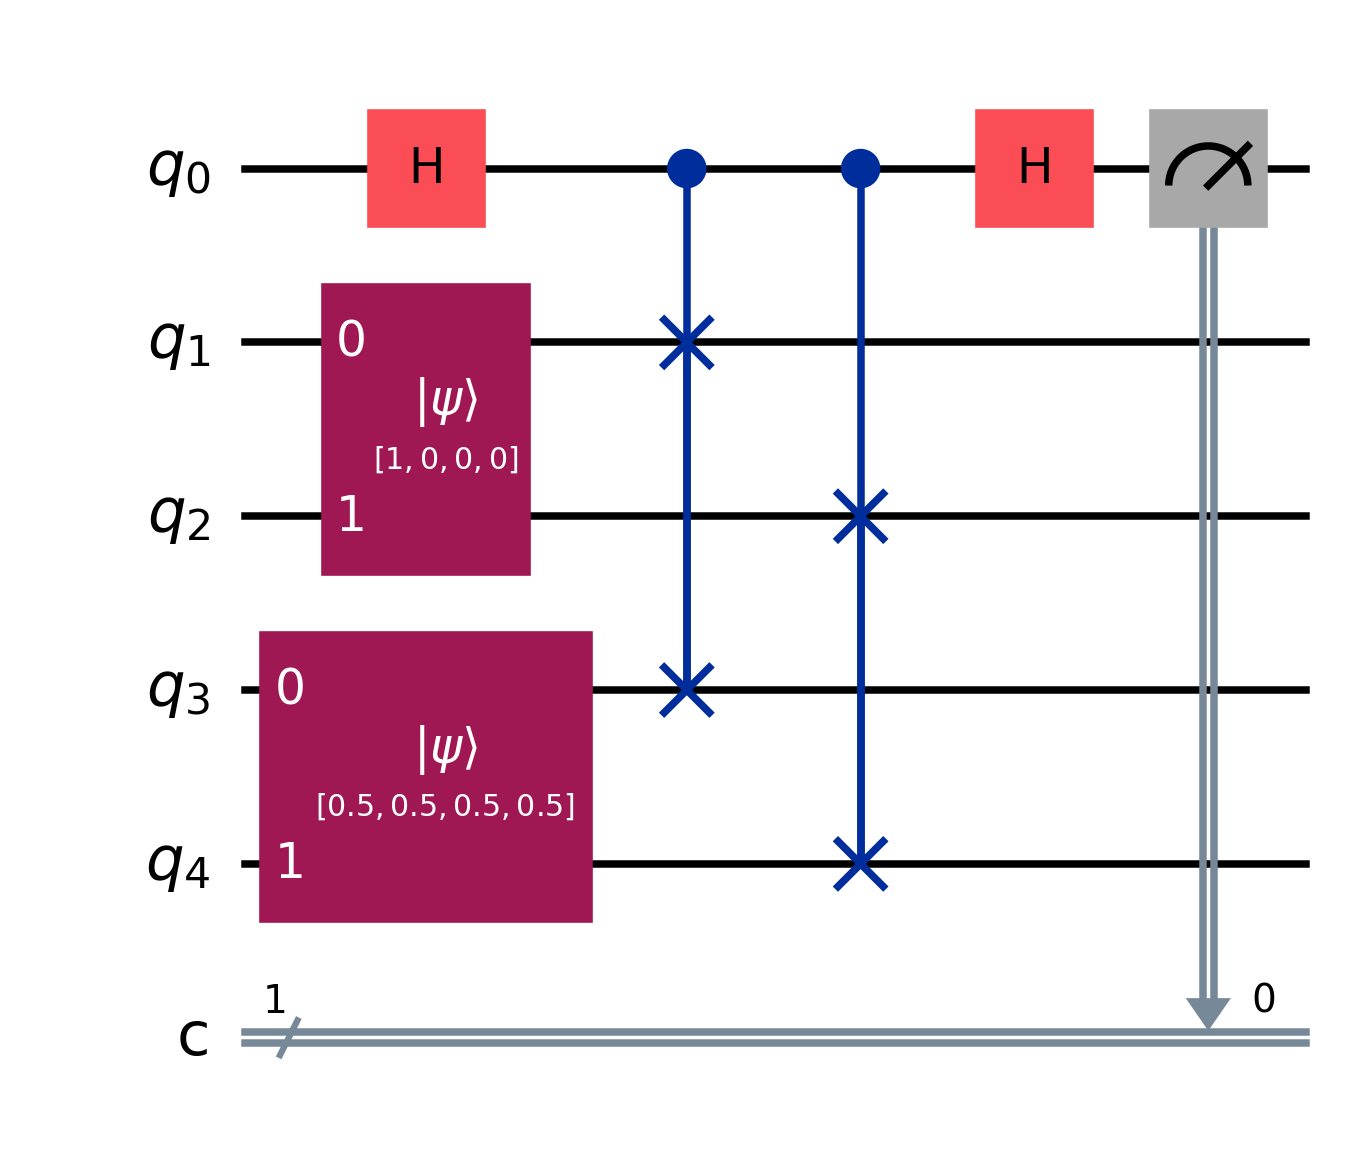
\includegraphics[width=0.7\linewidth]{figures/swap_test_circuit.png}
  \caption[Swap-test circuit]{Swap-test circuit for a four-dimensional example,
  in which each vector is amplitude-encoded into two qubits. The ancilla
  ($q_0$) is placed in superposition, controls a swap of the two encoded
  registers ($q_1 q_2$ and $q_3 q_4$), and is measured after a second Hadamard.
  The probability of reading the ancilla as zero gives the squared overlap of
  the two states, as in Equation~\ref{eq:swaptest}.}
  \label{fig:swaptest_circuit}
\end{figure}

\subsubsection{Qiskit Grover (Hardcoded Oracle)}
Grover's algorithm searches an unstructured collection of $N$ items for a marked
one using only about the square root of $N$ queries to an oracle, a quadratic
improvement over the $N$ comparisons a classical scan needs \cite{grover1996}.
Our engine implements the textbook circuit: it places an index register of
$\log_2 N$ qubits, with $N$ padded up to a power of two, into uniform
superposition, then repeats an oracle followed by a diffusion operator
$\lfloor\pi\sqrt{N}/4\rfloor$ times before measuring;
Figure~\ref{fig:grover_circuit} shows one such iteration for a four-element
index. The oracle flips the phase
of the target index and the diffusion step amplifies its amplitude, so the
measurement returns the marked index with high probability. The honest
difficulty is the oracle itself. For this to be a genuine search, the oracle
would have to compute, in superposition, which of the $N$ stored vectors is
closest to the query, which in turn requires loading all $N$ vectors into the
quantum state through a quantum random access memory, a device that addresses a
superposition of memory cells \cite{giovannetti2008qram}. No such hardware
exists at usable scale, and if instead the data has to be loaded one item at a
time the preparation alone costs $O(N)$, which erases the quadratic advantage
before the search even begins \cite{aaronson2015readfine}. We therefore make the
limitation explicit rather than hide it: the engine finds the nearest neighbour
classically and constructs an oracle that marks exactly that index. This
isolates the search step so that we can measure its oracle-call count and confirm
that it follows the $\lfloor\pi\sqrt{N}/4\rfloor$ curve, which is the scaling
claim we are actually testing, not an end-to-end speedup we are claiming to have
achieved.

\begin{figure}[ht]
  \centering
  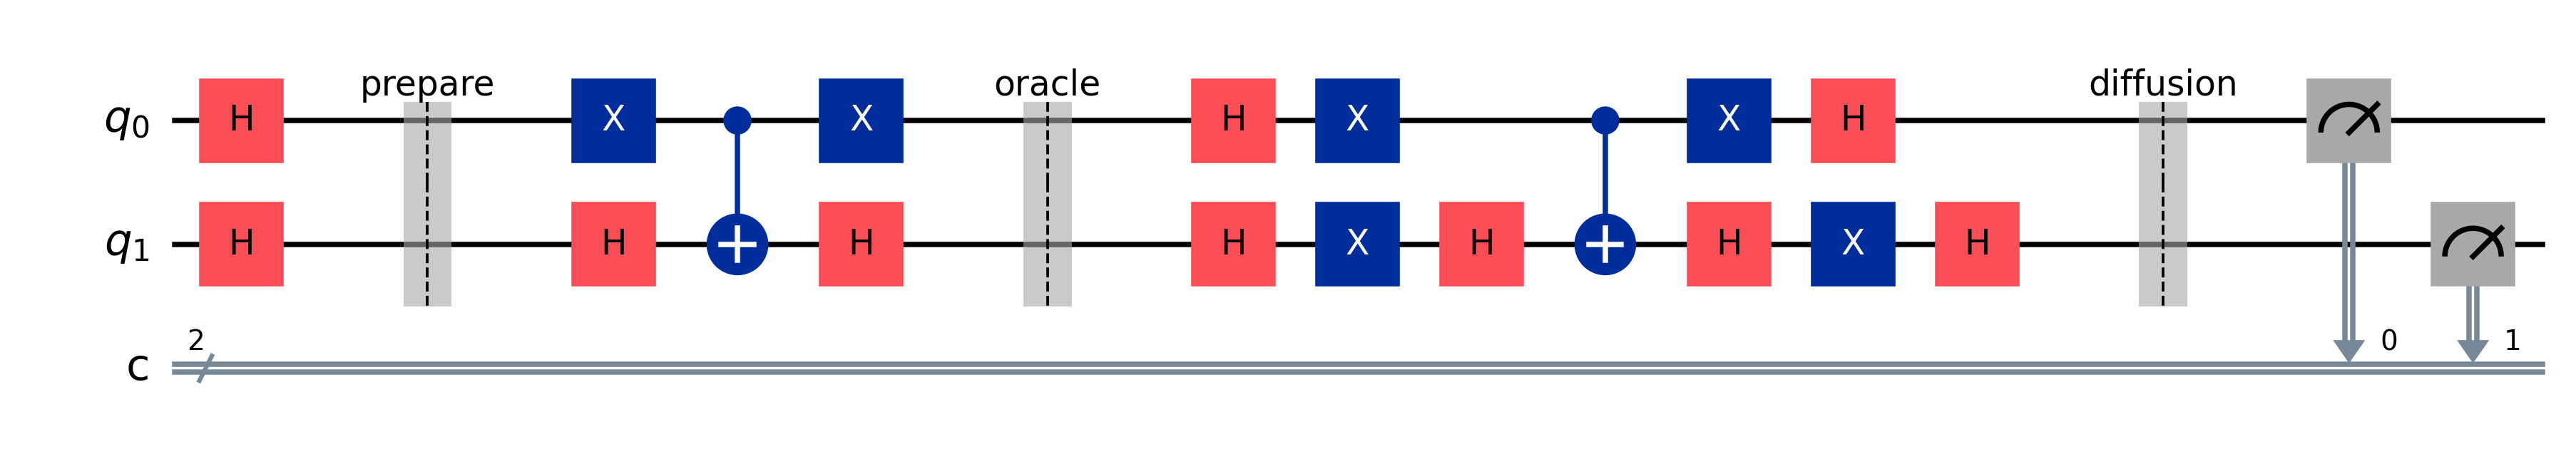
\includegraphics[width=\linewidth]{figures/grover_circuit.png}
  \caption[Grover circuit, one iteration]{One Grover iteration for a
  four-element index ($N=4$, two index qubits). After preparing a uniform
  superposition, the oracle flips the phase of the marked index and the
  diffusion operator amplifies its amplitude; the two qubits are then measured.
  The barriers separate the preparation, oracle, and diffusion phases.}
  \label{fig:grover_circuit}
\end{figure}

\subsubsection{Qiskit Grover with Quantum State Preparation}
The final Grover variant removes the one classical shortcut that the previous
engine kept. Instead of locating the nearest neighbour with a classical dot
product, it determines the target index quantum-mechanically: each stored vector
and the query are loaded with Qiskit state-preparation gates, a swap test
estimates their overlap, and the index with the highest measured overlap becomes
the one the Grover oracle marks. Everything after that, the superposition, the
oracle and diffusion iterations, and the final measurement, is identical to the
hardcoded variant. We include it to see what happens when the target selection
is itself made quantum, and therefore noisy, rather than exact. The outcome,
previewed here and quantified in the Results chapter, is that accuracy falls:
state preparation produces deep circuits, the per-candidate swap test carries the
same shot noise as the standalone swap-test engine, and any error in the quantum
target selection is then faithfully amplified by Grover, which has no mechanism
to recover once it has been pointed at the wrong index. This engine is thus the
most fully quantum of those we study and also the least accurate, a tension that
is itself one of the findings the project set out to document.

\subsubsection{Hybrid HNSW + Swap Test}
The hybrid engine is the one design in the study that tries to place the quantum
component where it might plausibly help rather than use it as a standalone
search. It runs in two stages. First the classical HNSW index retrieves a small
pool of candidates, by default the five nearest, cheaply narrowing the twenty
images down to a handful. The swap-test reranker then runs only on that pool,
scoring each surviving candidate against the query and reordering them. Because
the expensive quantum step is applied to a fixed-size shortlist instead of the
whole collection, the number of circuits no longer grows with the dataset: the
classical stage absorbs the $O(N)$ work and the quantum stage does a constant
amount of refinement on top. This mirrors the way approximate and exact stages
are already combined in production retrieval, where a fast approximate index
proposes candidates and a slower, more precise scorer reranks them, and it is the
most defensible place to insert a quantum estimator given that the swap test
offers no search speedup of its own. On our small collection the shortlist almost
always already contains the correct image, so the hybrid tracks the classical
baseline closely; its value here is architectural, showing the shape a useful
quantum contribution would take rather than a raw accuracy gain.

\subsubsection{IBM Hardware Validation}
To check that the quantum component is not merely a simulator artefact, we ran
the hybrid engine once on a real IBM quantum processor through the IBM Quantum
runtime, with the swap-test reranking executed on physical hardware rather than
the Aer simulator. This run is deliberately tiny. Vectors are truncated to just
two dimensions, the candidate pool is two images, and each circuit is measured
with thirty-two shots, a configuration small enough to fit within the limited
free-tier processor time and shallow enough that a noisy device can execute it at
all. It is a sanity check, not a scaling experiment: the aim is to confirm that
the encode, swap-test, and measure pipeline behaves on real hardware as it does
in simulation, and to expose honestly how much device noise and aggressive
truncation cost in accuracy. The resulting quality, reported with the other
measurements in the Results chapter, is far below the simulated engines and close
to chance, which is the expected consequence of two-dimensional vectors and
thirty-two shots on a noisy processor rather than a failure of the method. We
draw no scaling conclusions from it; its role is to ground the rest of the study,
which runs on a simulator, against at least one execution on a physical quantum
computer.

\section{Evaluation Metrics}
\label{sec:method:metrics}

% Define MRR formally, then define oracle calls. Explain why wall-clock is per-
% engine only - the simulator-time issue.

The primary measure of accuracy is the mean reciprocal rank (MRR), a standard
information-retrieval metric. For each query it rewards the engine with the
reciprocal of the rank at which the correct image appears: a correct image
ranked first scores one, ranked second one half, ranked fifth one fifth, and a
correct image that falls outside the top $k$ results returned, with $k$ fixed at
ten throughout, scores zero. Averaging this reciprocal rank over all queries
gives the MRR reported for an engine, as defined in Equation~\ref{eq:mrr}.
Because every engine is scored against the same ground-truth ranking and, as
established in Section~\ref{sec:method:embeddings}, the underlying similarity
measures induce identical orderings on unit vectors, a single MRR value can be
compared directly from one engine to the next.

\begin{equation}
\text{MRR} = \frac{1}{|Q|} \sum_{q \in Q} \frac{1}{\text{rank}_q},
\label{eq:mrr}
\end{equation}
where $\text{rank}_q$ is the position of the first relevant result for query
$q \in Q$ and $1/\text{rank}_q \coloneqq 0$ if no relevant result is in the top-$k$.

Accuracy alone does not capture why a quantum approach might ever be worth the
trouble, so we also record how each engine scales. The natural measure is the
operation count, the number of times an engine runs its core operation for a
single query, which is independent of the machine it runs on: a slow laptop and a
fast server execute the same number of iterations. The exhaustive engines, brute
force, FAISS flat, and the standalone swap test, perform one comparison or one
circuit per image and so scale as $O(N)$; HNSW traverses its graph in
$O(\log N)$; the hybrid does an $O(\log N)$ prefilter followed by a fixed number
$M$ of swap tests, $O(\log N + M)$; and Grover completes its search in
$\lfloor\pi\sqrt{N}/4\rfloor$ oracle cycles, $O(\sqrt{N})$. We store this figure
in the oracle-calls field of each result, and it is the only speed-like quantity
we compare across engines.

For the quantum engines we additionally record two circuit properties that
determine whether a circuit could run on real hardware. Circuit depth counts the
sequential layers of gates and is the main proxy for how much noise a physical
device would accumulate, since today's machines execute only a limited number of
layers reliably. Qubit count is the width of the circuit, which for the swap test
is the $1 + 2\lceil\log_2 d\rceil$ derived earlier. These fields are populated
only by the engines that build circuits; the classical engines leave them empty.
We deliberately do not compare wall-clock time across engines. The quantum
engines run on a simulator that reproduces quantum behaviour by manipulating an
exponentially large state vector on an ordinary CPU, so their runtimes mostly
measure the cost of that simulation rather than anything intrinsic to the
algorithm; comparing them with classical CPU timings would penalise the quantum
methods for the wrong reason. We therefore report wall-clock only within a single
engine, where it is meaningful, and never as a cross-engine ranking.

\section{Experimental Configuration}
\label{sec:method:config}

Table~\ref{tab:config} lists the parameter grid the benchmark sweeps. The
harness runs the full cartesian product of these values: every engine is
evaluated at each vector dimension, and the four quantum engines, which accept a
shot count, are additionally run at each shot setting, while the three classical
engines ignore shots and are run once per dimension. Each resulting
configuration is evaluated on all twenty queries. This produces fifteen
engine-and-shot configurations per dimension, three classical and four quantum at
three shot counts each, forty-five across the three dimensions, and nine hundred
individual query runs once multiplied by the twenty queries. The separate IBM
hardware validation contributes a further twenty runs, one per query, for a
stored total of nine hundred and twenty results. The layers parameter is held at
one throughout; the harness requires it but no engine enabled here uses it. Every
run is written to a PostgreSQL table together with its full parameter set, and
the database is dumped to a seed file committed alongside the code, so the entire
dataset can be reconstructed exactly rather than trusted as a one-off snapshot.

\begin{table}[ht]
  \centering
  \caption{Benchmark configuration grid.}
  \label{tab:config}
  \begin{tabular}{l p{7.2cm}}
    \toprule
    \textbf{Parameter} & \textbf{Values} \\
    \midrule
    Engines             & Brute-force cosine, FAISS flat, FAISS HNSW
                          (classical); swap test, Grover (hardcoded oracle),
                          Grover (quantum prep), hybrid HNSW + swap test
                          (quantum) \\
    Dimensions          & 64, 128, 256 \\
    Shots               & 512, 1024, 2048 (quantum engines only) \\
    Layers              & 1 \\
    Top-$k$             & 10 \\
    \bottomrule
  \end{tabular}
\end{table}

\section*{Use of AI Tools}
\label{sec:method:ai}
\addcontentsline{toc}{section}{Use of AI Tools}

% MANDATORY per FENS handbook \S1.1. Be specific - generic disclaimers fail
% the originality check. State which tools were used for which tasks.

This project made use of AI assistants, specifically Claude Code and ChatGPT, as
productivity tools during development and writing. Their role was to accelerate
well-defined, labour-intensive tasks under the authors' direction, not to
originate the work. Concretely, the tools assisted with generating and
refactoring routine code, reviewing changes and helping locate bugs during the
code audit, drafting prose that the authors then revised, and rendering diagrams
from layouts the authors specified.

The intellectual core of the project is the authors' own. The system
architecture, including the strategy-pattern engine interface and the five-phase
pipeline, the selection and configuration of the search engines, the design of
the benchmark and its research questions, and the interpretation of the results
were reasoned through and decided by the authors. Every benchmark figure reported
here was produced by our own experimental runs, and every external reference was
verified by the authors against its primary source before it was cited.

The authors take full responsibility for the correctness, originality, and
verification of all code, data, and conclusions in this report. Where AI tools
contributed text or code, that output was read, checked, and where necessary
corrected and rewritten by the authors, who treat it as a draft to be
scrutinised rather than as an authority to be trusted.
